\begin{figure}[htbp]
 \centering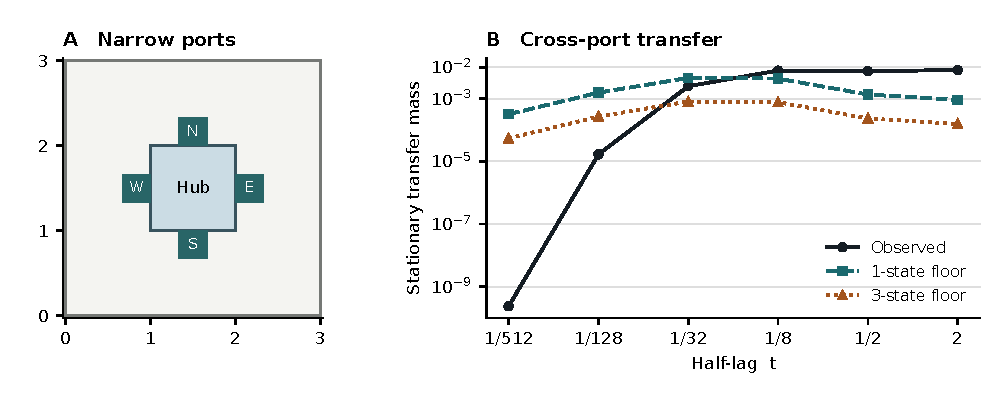
\includegraphics[width=.97\linewidth]{junction.pdf}
 \caption{Equilibrium diffusion with separated ports. The four dark patches in A are the measured ports. Panel B uses \(n=18\), \(D_x=D_y=1\), and \(w=1/3\). Observed mass below a floor excludes the corresponding hub budget. At half-lag \(1/32\) the data still exclude one state; at \(1/8\) the displayed floors both fall below the observation.}
 \label{fig:diffusion}
\end{figure}

For separated ports, the lower bound on the state count reached four in 19 of 42 configurations, three in two, two in three, and one in 18. For full-width ports it remained one in all 42. The trend with half-lag is visible in Figure~\ref{fig:diffusion}. At \(n=18,t=1/128\) in the isotropic separated case the observed mass was \(1.674\cdot10^{-5}\), compared with \(2.682\cdot10^{-4}\) required by any three-state hub and \(2.768\cdot10^{-3}\) predicted by repeating the one-step six-label kernel. In the full-width case at the same resolution and lag, the global prediction \(0.02811\) also exceeded the observed \(0.01827\), but the local one-state floor was only \(0.01145\). This discrepancy cannot be assigned to the hub by the all-pair test.

Enforcing the occupancy constraints increased the certified count in one of 84 configurations. At \(n=36,D_y=1/4,w=1/3,t=1/32\) the observed mass \(2.478\cdot10^{-4}\) lay between the relaxed and exact three-state floors, \(2.387\cdot10^{-4}\) and \(2.538\cdot10^{-4}\). At \(n=18\) in that same geometry the exact floor lay just below the observation. Thus the stronger four-state conclusion at this lag is sensitive to spatial resolution.
